%% osm-applications.tex
%%


\section{Applications}

\frame[plain]{  \heading{Plan de la Présentation}
\ecmsetupplan
\begin{itemize}
  \item[\small $\Diamond$] Introduction
  \item[\small $\Diamond$] Fonctionnement
  \item[\small $\Diamond$] {\color{purple}\textbf{Applications}}
  \item[\small $\Diamond$] Conclusions
\end{itemize}
}



%% http://www.foss4g2007.org/presentations/view.php?abstract_id=56


\frame { \heading{Utilisations des données} \vfil

  %% http://wiki.openstreetmap.org/index.php/Fr:Using_OpenStreetMap
  
  %% http://fredericbonifas.free.fr/osm.html

  %% http://wiki.navit-project.org/images/thumb/f/fa/FBZH-gtk.png/800px-FBZH-gtk.png
  
  \begin{minipage}{0.8\textwidth}
  \begin{itemize}
  \item guidage temps réel (applications: pyroute, navit, GPSDrive,
    gosmore, roadnav) 
  \item cartes et applications de routage thématiques
    \begin{itemize}
    \item spécifique vélo ou piéton ou bâteau
    \item carte des châteaux d'une zone viticole
    \item préparation d'un \textit{pub crawl}
    \end{itemize}
  \item utiliser les données dans des simulateurs
    \begin{itemize}
    \item existe pour FlightGear (avec terragear)
    % TODO Inclure Image
    \item Dresden en 3D
    % TODO Inclure image
    \end{itemize}
  \item permet un réalisme troublant
    \begin{itemize}
    \item localisations des boîtes aux lettres, points de recyclage,
      toilettes, bornes SOS
    \end{itemize}
  \item insérer votre idée ici: les données sont libres!
  \end{itemize}
  \end{minipage} %
  \begin{minipage}{0.19\textwidth}
    \includegraphics[width=1.5cm]{figures/200px-Gpsdrive_ipaq_screenshot-map-z11}
    \vskip 1cm

    \includegraphics[width=1.5cm]{figures/240px-Now_turn_right2}
    \vskip 1cm
    
    \includegraphics[width=1.5cm]{figures/240px-Osmroads1}
    \vskip 1cm
  \end{minipage}
}

\frame{ \heading{Créer une carte personnalisée}  \vfill
  \begin{minipage}{0.45\textwidth}
    \begin{itemize}
    \item Service officiel (onglet ``Export'')
    \item Carte statique (PDF, SVG, PNG, XML)
    \item Carte dynamique (HTML embarquable)
    \end{itemize}
  \end{minipage} \quad %
  \begin{minipage}{0.49\textwidth}
    \includegraphics[width=\textwidth]{figures/OSM-export}
  \end{minipage}
}

\frame{ \heading{\'Edition en ligne}  \vfill
  \begin{minipage}{0.45\textwidth}
    POTLACH
    \begin{itemize}
    \item Service officiel (onglet ``Edit'')
    \item Coordonnées synchronisées avec la vue
    \item Validation manuelle ou automatique
    \item Accès aux données GPS
    \end{itemize}
  \end{minipage} \quad %
  \begin{minipage}{0.49\textwidth}
    \includegraphics[width=\textwidth]{figures/potlatch}
  \end{minipage}
}

\frame{ \heading{\'Edition hors-ligne}  \vfill
  \begin{minipage}{0.45\textwidth}
    JOSM
    \begin{itemize}
    \item Plus riche
    \item Plus souple
    \item Plugins variés
    \end{itemize}
    \end{minipage} \quad %
  \begin{minipage}{0.49\textwidth}
    \includegraphics[width=\textwidth]{figures/JOSM}
  \end{minipage}
}

\frame{ \heading{Outils de validation}  \vfill

\begin{itemize}
\item plugin validator
\item Keepright  % http://keepright.ipax.at
\item Osmose  % http://osmose.openstreetmap.fr
\item OpenStreetBugs % http://openstreetbugs.appspot.com/
\item MapCompare  % http://tools.geofabrik.de/mc/
\item OSM Inspector % http://tools.geofabrik.de/osmi/
\item moteurs de routage
\end{itemize}
}

\frame{ \heading{Réalisation carte municipale}  \vfill
  \begin{minipage}{0.45\textwidth}
MapOSMatic
\begin{itemize}
\item Carte de la ville
\item Index des noms
\end{itemize}
  \end{minipage} \quad %
  \begin{minipage}{0.49\textwidth}
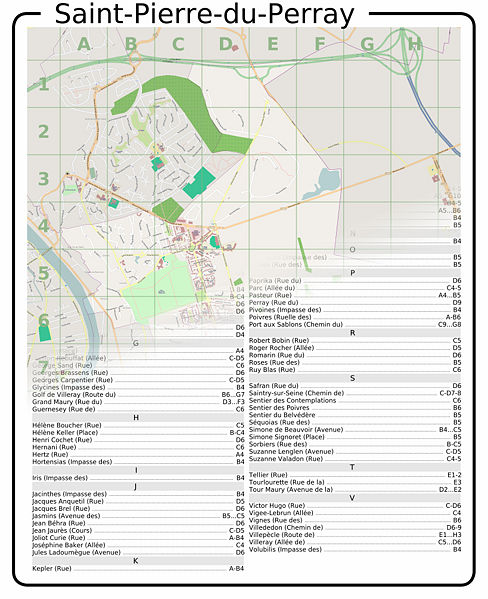
\includegraphics[width=\textwidth]{figures/MapOSMatic-SaintPierreDuPerray}
  \end{minipage}
}

\frame{ \heading{Routage et guidage}  \vfill
  \begin{minipage}{0.45\textwidth}
Gosmore
\begin{itemize}
\item Carte embarquée
\item Affichage POI
\item Routage (3D)
\end{itemize}
\begin{itemize}
\item Windows CE
\item Linux Maemo
\end{itemize}
  \end{minipage} \quad %
  \begin{minipage}{0.49\textwidth}
    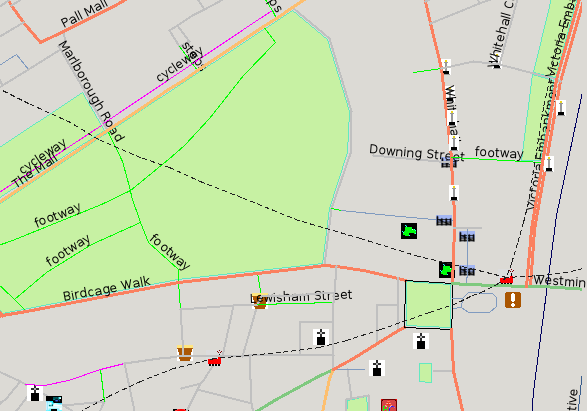
\includegraphics[width=0.8\textwidth]{figures/Gosmore}
\par
    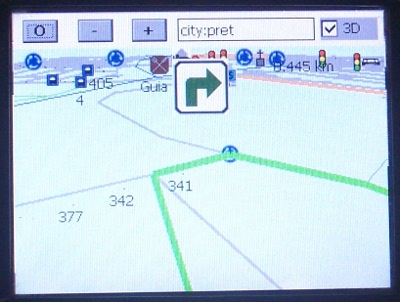
\includegraphics[width=0.8\textwidth]{figures/Gosmore3D}
  \end{minipage}
}

\frame{ \heading{Réalisation carte spécialisée}  \vfill
Chimère %http://redmine.peacefrogs.net/projects/show/chimere

  \begin{minipage}{0.45\textwidth}
    \begin{itemize}
      \item Association
      \begin{itemize}
        \item écologiste
        \item commerçants
        \item utilisateurs
      \end{itemize}
      \item Gestion des contributeurs
      \item Modération
      \item Liens avec OSM
    \end{itemize}

\begin{minipage}{0.70\textwidth}
\tiny
Crédits

Licence: \href{http://creativecommons.org/licenses/sa/1.0/}{CC-sa}
  \end{minipage} \quad %
  \begin{minipage}{0.20\textwidth}

\includegraphics[height=3ex]{figures/sa}
  \end{minipage}

  \end{minipage} \quad %
  \begin{minipage}{0.49\textwidth}
    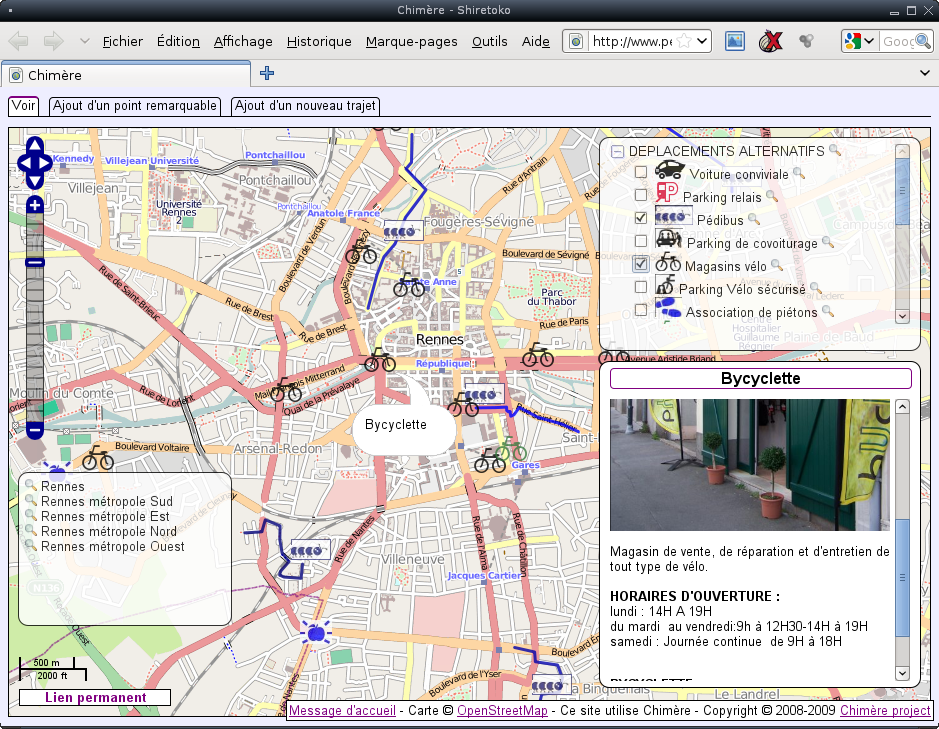
\includegraphics[width=\textwidth]{figures/chimere}
  \end{minipage}
}


\frame{ \heading{Utilisation sur terminal mobile} \vfil
  \begin{tikzpicture}[remember picture,overlay,font={\footnotesize},text
    width=2cm,text centered]
   \node[xshift=1cm,yshift=-4cm] at (current page.north west) {\includegraphics[width=7cm]{figures/osm-N800}};
   \node[xshift=-1cm,yshift=-3cm] at (current page.north east) {\includegraphics[height=5cm]{figures/OSM-garmin}};
   \node[xshift=-4.7cm,yshift=3.5cm] at (current page.south east) {\includegraphics[height=5cm]{figures/OSM-garmin-etrex}};
\end{tikzpicture}
}



\frame{ \heading{Utilisation sous Android} \vfil

}


%% http://www.geographie.uni-bonn.de/karto/osm-3d/screenshots.en.htm

\frame{ \heading{Réalisations artistiques}  \vfill

  \begin{minipage}{0.45\textwidth}
``Streets Clock''

Un plan de ville qui donne l'heure.
    \vskip 1cm
  \begin{minipage}{0.70\textwidth}
\tiny
Design: Fluid Forms, John Briscella

Photo: Alexander Karelly, Lupispuma

Licence: \href{http://creativecommons.org/licenses/by/2.0/deed.fr}{CC-by}

  \end{minipage} \quad %
  \begin{minipage}{0.20\textwidth}

\includegraphics[height=3ex]{figures/by}
  \end{minipage}
  \end{minipage} \quad %
  \begin{minipage}{0.49\textwidth}
    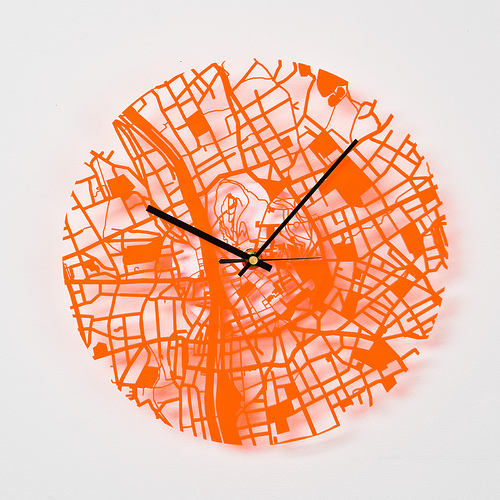
\includegraphics[width=\textwidth]{figures/streets_clock}
  \end{minipage}
}

\frame{ \heading{Réalisations artistiques}  \vfill

  \begin{minipage}{0.45\textwidth}
Un plan... à manger
    \vskip 1cm
  \begin{minipage}{0.60\textwidth}
\tiny
Gâteau SOTM 2009

Photo: Pierre-Luc Beaudoin

Licence: \href{http://creativecommons.org/licenses/by-sa/2.0/}{CC-by-sa}

  \end{minipage} \quad %
  \begin{minipage}{0.30\textwidth}
\includegraphics[height=3ex]{figures/cc-by-sa}
  \end{minipage}
  \end{minipage} \quad %
  \begin{minipage}{0.49\textwidth}
    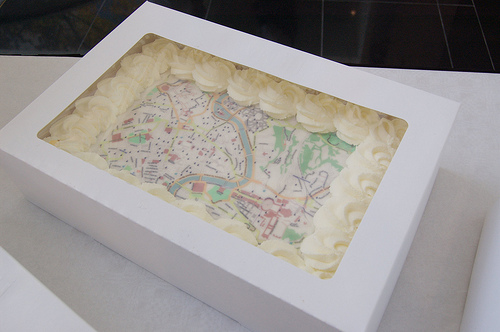
\includegraphics[width=0.8\textwidth]{figures/cake_sotm2009_1}
\par
    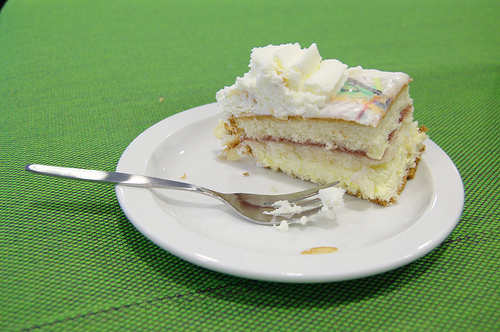
\includegraphics[width=0.8\textwidth]{figures/cake_sotm2009_2}
  \end{minipage}

}


%% EOF
